\subsection{Surface Reconstruction}

\begin{figure*}[t!]
	\centering
	\begin{subfigure}[b]{0.48\linewidth}
		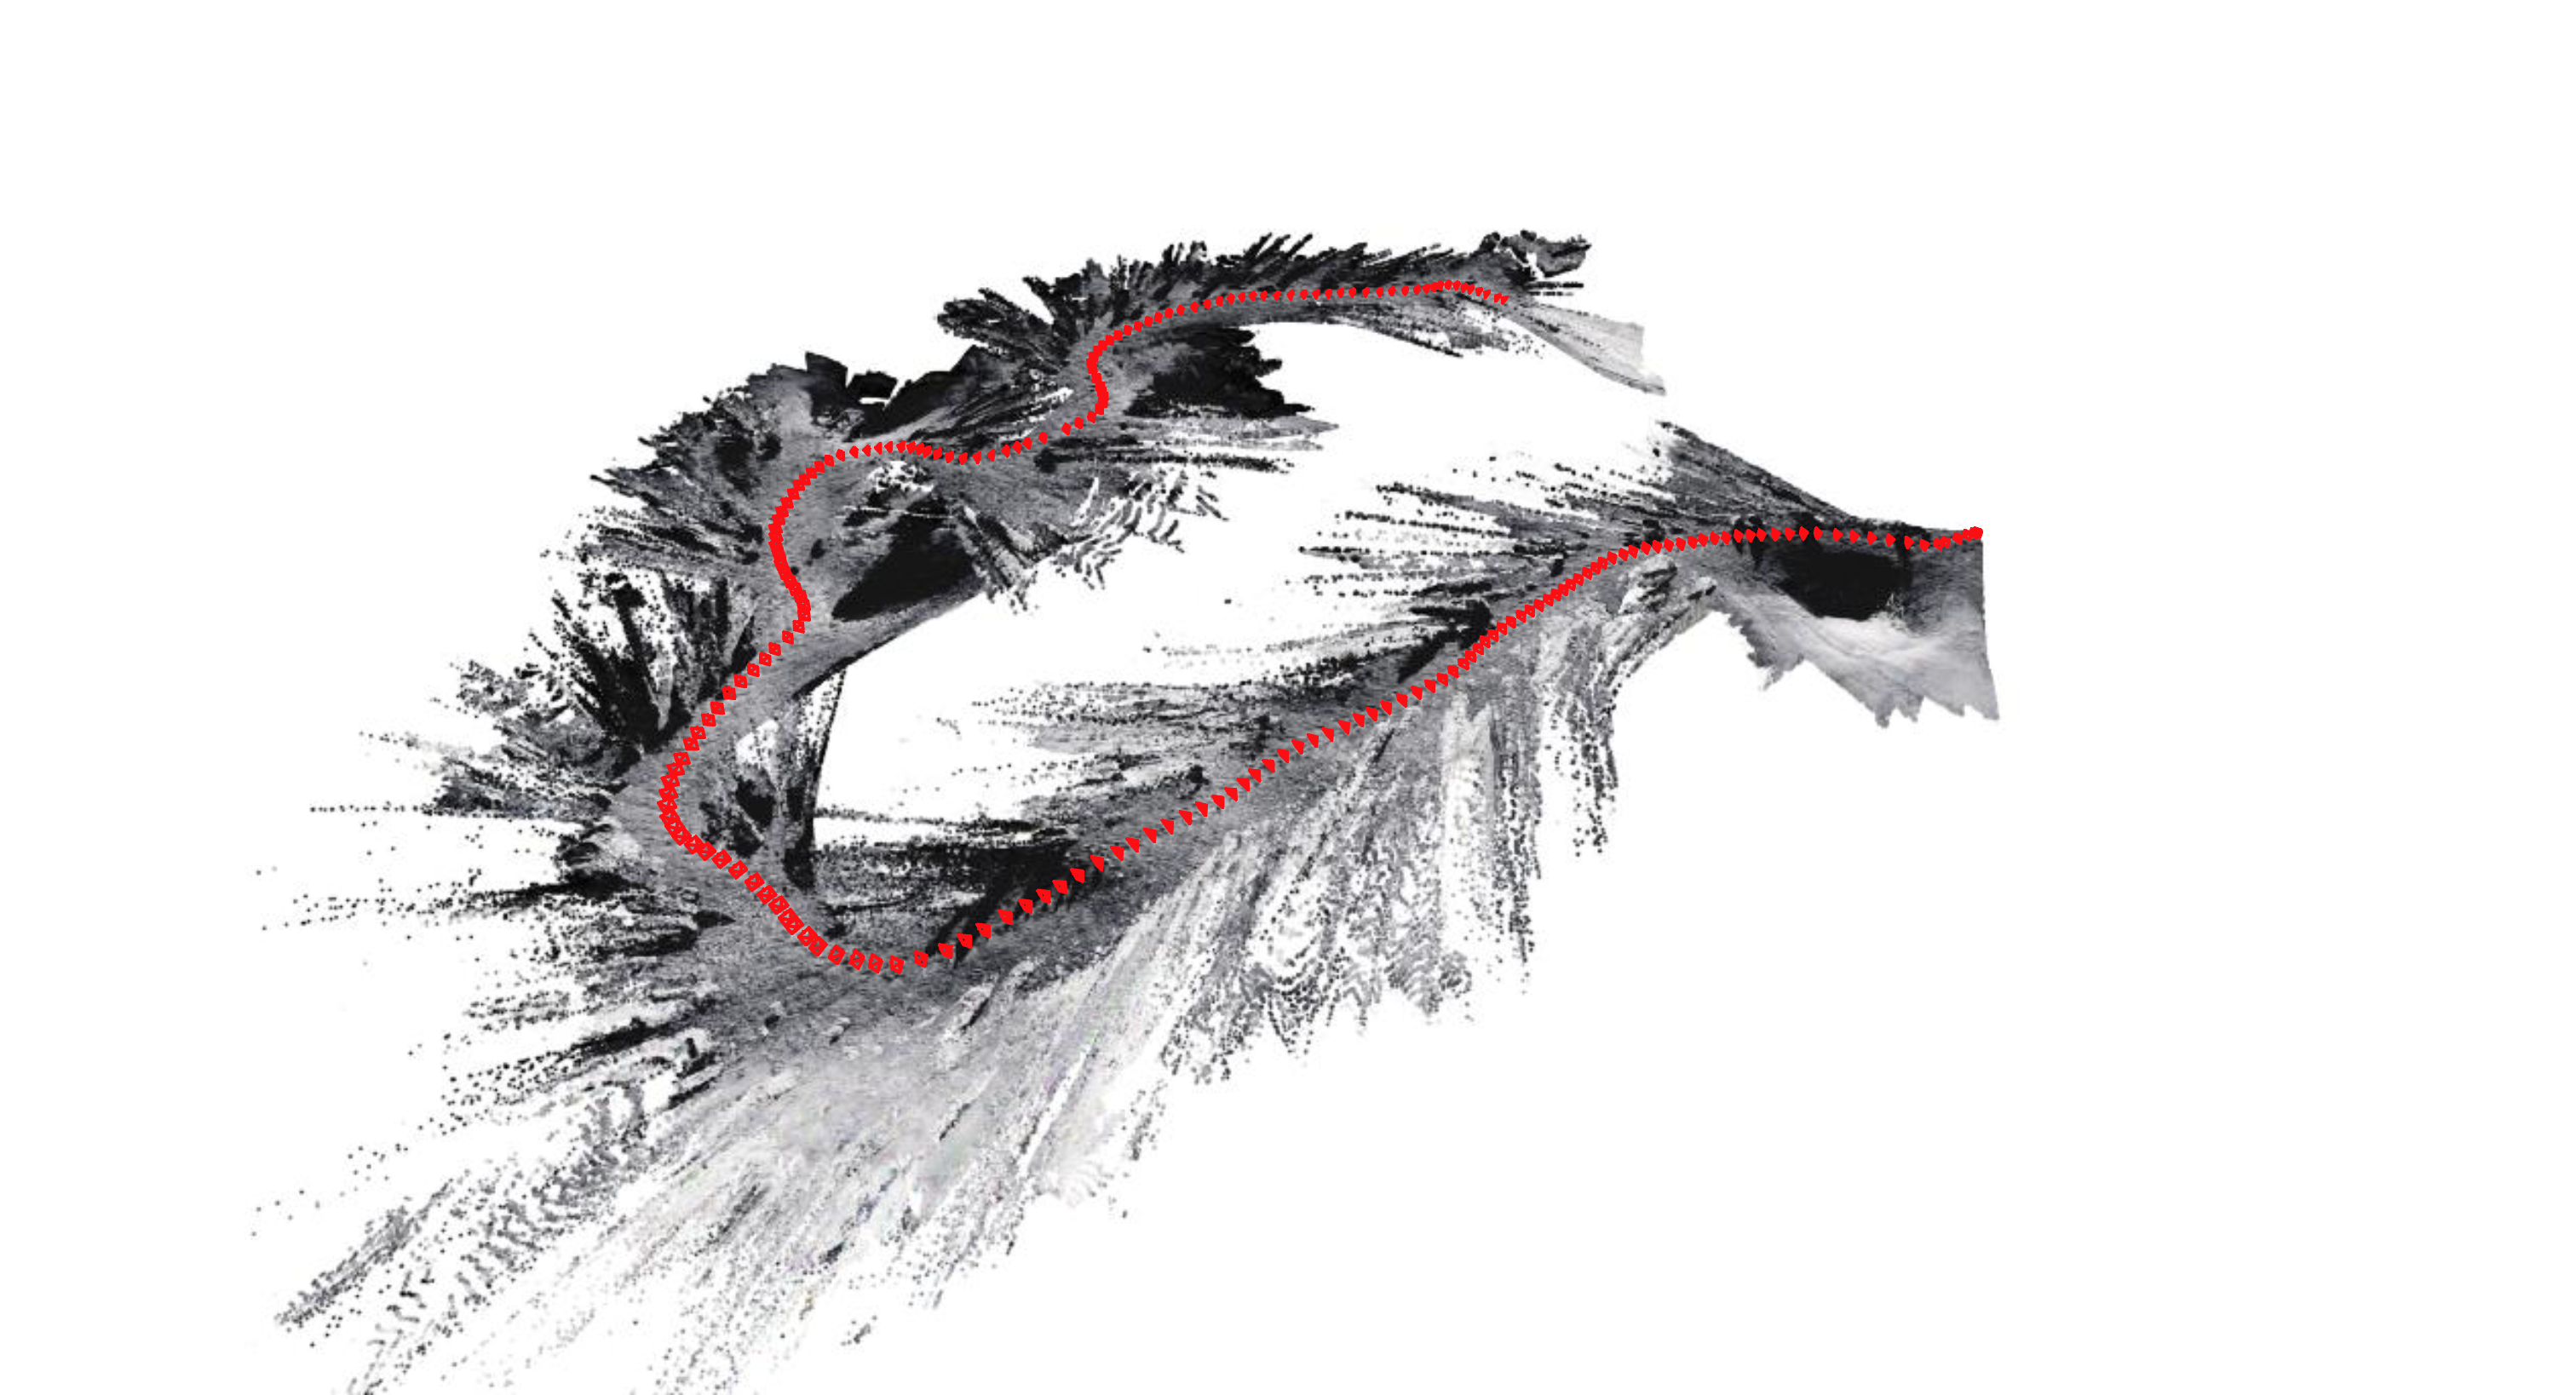
\includegraphics[width=\linewidth]{figures/3dgs/render-1.png}
	\end{subfigure}
	\hfill
	\begin{subfigure}[b]{0.48\linewidth}
		\includegraphics[width=\linewidth]{figures/3dgs/render-2.png}
	\end{subfigure}
	\vspace{1em}
	\begin{subfigure}[b]{0.48\linewidth}
		\includegraphics[width=\linewidth]{figures/3dgs/render-3.png}
	\end{subfigure}
	\hfill
	\begin{subfigure}[b]{0.48\linewidth}
		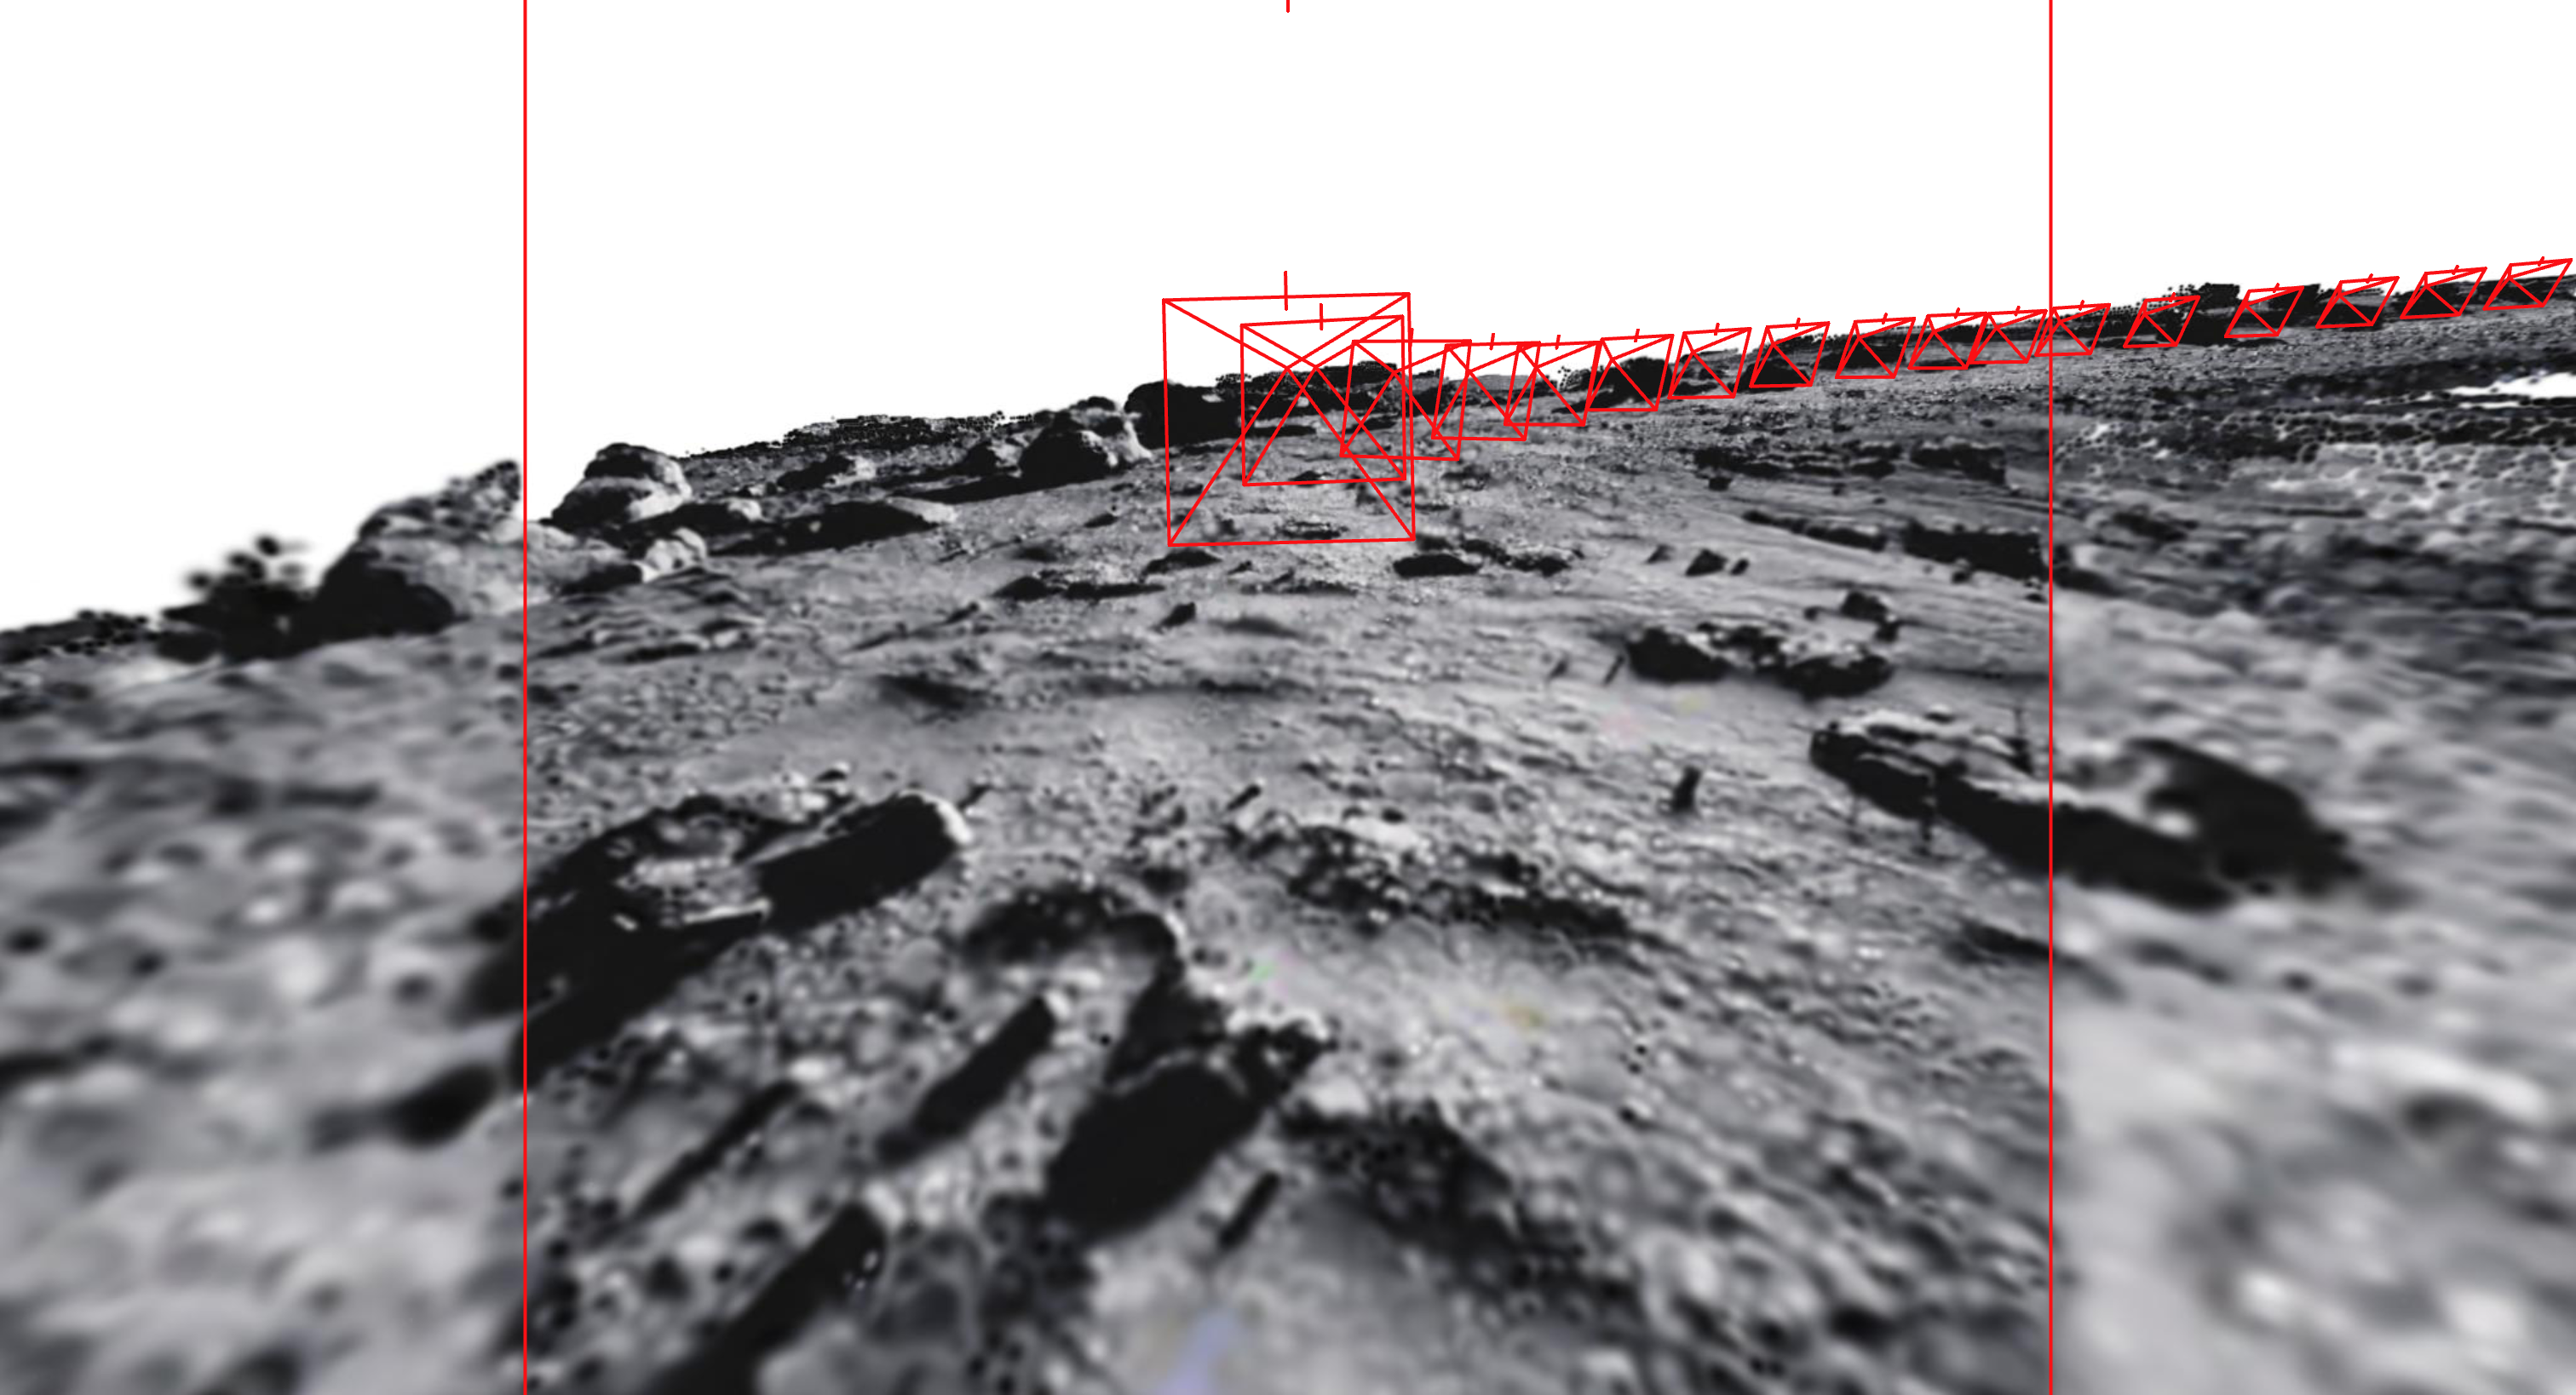
\includegraphics[width=\linewidth]{figures/3dgs/render-4.png}
	\end{subfigure}
	\caption{\bfseries Qualitative results of the real-time 3DGS reconstruction.}
	\label{fig:surface_recon_qual}
\end{figure*}

We implemented our own real-time 3DGS reconstruction pipeline based on Splat-SLAM~\cite{sandstrom_splat-slam_2024} and a point cloud mapping baseline. Our implementation uses ground truth pose information and prior terrain knowledge (without rocks or craters) to initialize the scene. For each new image, we use ground truth segmentation to remove sky regions and tag Gaussians with semantic information, compute depth using our depth estimation models, add new Gaussians to the scene based on RGB and depth information (computing their scale), and optimize the scene in the background using past images. The optimization objective includes L1 RGB and depth losses, penalties for Gaussian density above the surface, Structural Similarity Index Measure (SSIM) loss to ensure the reconstructed images maintain proper structural relationships and perceptual quality compared to the input images, and additional Gaussian regularization terms.
Currently, we do not implement splitting and merging of Gaussians, but we remove Gaussians that are far from the prior terrain.
\Cref{fig:splat-slam} shows the steps of the pipeline using the custom Open3D environment.

\Cref{fig:map_3dgs} shows the 3DGS and point cloud map reconstructions on the Open3D environment, Table~\ref{tab:surface_reconstruction} shows the surface reconstruction and rock detection results, and \cref{fig:novel_views} shows a top view of the 3DGS map. Gaussian splatting with RAFT-Stereo depth outperforms the point cloud baseline in reconstruction accuracy, likely due to its joint optimization over depth and RGB data across multiple views. This demonstrates the potential of neural scene representations for SLAM applications. When ground truth depth is used, the point cloud baseline performs slightly better. We attribute this to our current approach of reconstructing the mesh from the centers of the Gaussians rather than accounting for their density.

In both cases, most errors occur around rocks, which are often dark and hard to distinguish from the sky, making depth estimation challenging. Rock detection performance is comparable between methods, while the point cloud baseline yields lower height error—-possibly due to differences in how the mesh is extracted from the 3DGS map.

\begin{table*}[h]
	\centering
	\small
	\caption{\bfseries Surface reconstruction results. TO BE UPDATED}
	\label{tab:surface_reconstruction}
	\begin{tabular}[t]{|lrrrrrr|}
		\hline
		\multirow{2}{*}{\textbf{Metric}}               &
		\multicolumn{1}{c}{\textbf{Accuracy}}          &
		\multicolumn{1}{c}{\textbf{Completion}}        &
		\multicolumn{1}{c}{\textbf{Precision}}         &
		\multicolumn{1}{c}{\textbf{Recall}}            &
		\multicolumn{1}{c}{\textbf{F-Score}}           &
		\multicolumn{1}{c|}{\textbf{Height Error}}
		\\
		\multicolumn{1}{|c}{}                          &
		\multicolumn{1}{c}{\textbf{[cm] $\downarrow$}} &
		\multicolumn{1}{c}{\textbf{[cm] $\downarrow$}} &
		\multicolumn{1}{c}{\textbf{[\%] $\uparrow$}}   &
		\multicolumn{1}{c}{\textbf{[\%] $\uparrow$}}   &
		\multicolumn{1}{c}{\textbf{[\%] $\uparrow$}}   &
		\multicolumn{1}{c|}{\textbf{[cm] $\downarrow$}}
		\\
		\hline\hline
		\multicolumn{7}{|l|}{\textbf{3DGS}}                                                       \\
		Rock                                           & 61.3  & 27.0 & 13.7 & 26.7 & 18.1 & 15.4 \\
		Regolith                                       & 12.9  & 28.0 & 60.0 & 66.8 & 63.2 & 8.2  \\
		Crater                                         & 941.1 & 27.0 & 9.9  & 15.3 & 12.0 & 74.6 \\
		All                                            & 17.5  & 25.8 & 53.2 & 60.7 & 56.7 & 10.4 \\
		\multicolumn{7}{|l|}{\textbf{ + Ground Truth Depth and Segmentation}}                     \\
		Rock                                           & 61.3  & 27.0 & 13.7 & 26.7 & 18.1 & 15.4 \\
		Regolith                                       & 12.9  & 28.0 & 60.0 & 66.8 & 63.2 & 8.2  \\
		Crater                                         & 941.1 & 27.0 & 9.9  & 15.3 & 12.0 & 74.6 \\
		All                                            & 17.5  & 25.8 & 53.2 & 60.7 & 56.7 & 10.4 \\
		\hline
		\multicolumn{7}{|l|}{\textbf{Point Cloud}}                                                \\
		Rock                                           & 61.3  & 27.0 & 13.7 & 26.7 & 18.1 & 15.4 \\
		Regolith                                       & 12.9  & 28.0 & 60.0 & 66.8 & 63.2 & 8.2  \\
		Crater                                         & 941.1 & 27.0 & 9.9  & 15.3 & 12.0 & 74.6 \\
		All                                            & 17.5  & 25.8 & 53.2 & 60.7 & 56.7 & 10.4 \\
		\multicolumn{7}{|l|}{\textbf{+ Ground Truth Depth and Segmentation}}                      \\
		Rock                                           & 61.3  & 27.0 & 13.7 & 26.7 & 18.1 & 15.4 \\
		Regolith                                       & 12.9  & 28.0 & 60.0 & 66.8 & 63.2 & 8.2  \\
		Crater                                         & 941.1 & 27.0 & 9.9  & 15.3 & 12.0 & 74.6 \\
		All                                            & 17.5  & 25.8 & 53.2 & 60.7 & 56.7 & 10.4 \\
		\hline
	\end{tabular}
\end{table*}



\begin{table}[h]
	\centering
	\small
	\caption{\bfseries Memory usage for 3DGS.}
	\label{tab:memory_usage}
	\begin{minipage}[t]{0.48\linewidth}
		\centering
		\begin{tabular}[t]{|lr|}
			\hline
			\textbf{GPU VRAM} & 1017 MB \\\hline\hline
			\textbf{3DGS}     & 793 MB  \\
			~~Means           & 170 MB  \\
			~~Scales          & 170 MB  \\
			~~Rotations       & 227 MB  \\
			~~Opacities       & 56 MB   \\\hline
			\textbf{Strategy} & 224 MB  \\
			~~Radii           & 56 MB   \\
			~~Labels          & 56 MB   \\
			~~Gradients       & 56 MB   \\
			~~Counts          & 56 MB   \\\hline
		\end{tabular}
	\end{minipage}%
	\begin{minipage}[t]{0.48\linewidth}
		\centering
		\begin{tabular}[t]{|lr|}
			\hline
			\textbf{System RAM} & 1900 MB \\\hline\hline
			~~RGBs              & 1200 MB \\
			~~Depths            & 400 MB  \\
			~~Masks             & 200 MB  \\
			~~Labels            & 100 MB  \\
			\hline
		\end{tabular}
	\end{minipage}
\end{table}
